\documentclass[conference]{IEEEtran}

\usepackage{amsmath}
\usepackage{graphicx}
\usepackage{booktabs}
\usepackage{float}
\usepackage{placeins}
\usepackage{textcomp}
\usepackage{url}
\usepackage{hyperref}
\usepackage{multirow}

\title{\vspace{-0.8cm}Spatial Feature Engineering for Urban Civic Complaint Prioritization: A Hybrid Synthetic and Real-World Evaluation}

\author{

\IEEEauthorblockN{
Dr. Ashish Kumar Kesarwany$^{1}$ \quad
Pratham Kashyap$^{2}$ \quad
Harshit Chugh$^{2}$ \quad
Aditya Priyadarshi$^{3}$ \\
Anusha Gupta$^{3}$ \quad
Viya Sharma$^{3}$ \quad
Ashwin Joseph$^{2}$
}

\vspace{0.2cm}

\IEEEauthorblockA{
$^{1}$School of Applied Sciences and Language (SASL), VIT Bhopal University, India
}

\IEEEauthorblockA{
$^{2}$School of Computing Science Engineering and Artificial Intelligence (SCAI), VIT Bhopal University, India
}

\IEEEauthorblockA{
$^{3}$School of Computer Science Engineering (SCOPE), VIT Bhopal University, India
}

\vspace{0.15cm}

\IEEEauthorblockA{
\small
ashishkumarkesarwany@vitbhopal.ac.in \\
pratham.23bai10455@vitbhopal.ac.in \\
aditya.23bce10821@vitbhopal.ac.in \\
anusha.23bce10866@vitbhopal.ac.in \\
harshit.23bai10101@vitbhopal.ac.in \\
viya.23bce11351@vitbhopal.ac.in \\
ashwin.23bcy10005@vitbhopal.ac.in
}

}


\begin{document}

\maketitle

\begin{abstract}
Automated prioritization of civic complaints is increasingly important for municipal teams that must triage large volumes of waste, road, lighting, drainage, and water-supply reports. We investigate whether spatial density information can improve this triage process through a combined classification and clustering pipeline. The framework combines radius-based priority labeling, K-nearest neighbor (KNN) density feature extraction, and DBSCAN hotspot detection in a modular workflow. Using a synthetic Bhopal dataset for controlled spatial experimentation, we find that spatial features improve the Decision Tree baseline from 72.9\% to 87.4\% accuracy, while XGBoost reaches 90.9\%. External validity is assessed by training directly on 5,469 NYC~311 service requests labeled via observed resolution outcomes, where XGBoost achieves 95.7\% cross-validated accuracy and 0.903 macro F1. We also show that direct model transfer remains difficult: Random Forest performs best in zero-shot Bhopal-to-NYC transfer at 65.3\%, while XGBoost drops to 38.7\%. Finally, DBSCAN identifies 28 controlled Bhopal hotspots and 99 NYC~311 hotspots, linking ticket-level prioritization with area-level resource planning.
\end{abstract}

\section{Introduction}

The acceleration of urban growth globally has escalated the strain on municipal services, manifested in a rising volume of public grievances concerning waste, damaged roads, and utility disruptions. Resolving these community reports promptly is vital to sustaining public safety and structural integrity in modern cities~\cite{batty2013big}. Yet, contemporary municipal dashboards typically process service requests in isolation or through static rules, overlooking localized spatial contexts and compound urgency~\cite{kontokosta2017urban}.

Geospatially-tagged complaints generated by citizens through platforms like NYC 311~\cite{minkoff2016nyc311} or regional municipal portals offer valuable location intelligence that is rarely exploited for triage. A cluster of adjacent complaints often points to broader structural failures---such as recurring pipeline ruptures within a specific neighborhood---warranting higher priority than isolated complaints. However, standard city management pipelines evaluate reports individually, discarding spatial dependency signals~\cite{goodchild2007citizens}.

Methods in urban computing~\cite{zheng2014urban} and machine learning~\cite{bishop2006pattern} have facilitated analytical strategies for civic administration. While spatial algorithms like DBSCAN~\cite{ester1996dbscan} are common for hotspot mapping, and tree ensembles~\cite{breiman1984classification,breiman2001random} excel at representing complex feature dependencies, there is a gap in research that systematically isolates and measures how much spatial density features improve priority classification under controlled experimental conditions.

This paper proposes a spatially-aware machine learning framework that integrates KNN-based density features with supervised classification for civic complaint prioritization. The key insight is that spatial density---capturing localized complaint concentration---serves as a meaningful predictive feature when combined with domain-knowledge features such as complaint category and resolution status.

The main contributions of this work are:
\begin{itemize}
    \item A domain-knowledge-based labeling scheme that incorporates spatial context through same-category neighbor analysis, avoiding circular label-feature dependencies.
    \item A KNN-based density feature engineering approach that captures spatial complaint concentration patterns.
    \item A comprehensive experimental evaluation with 5-fold cross-validated ablation study demonstrating the impact of spatial features.
    \item Integration of DBSCAN-based hotspot detection for identifying critical urban zones requiring targeted resource allocation.
\end{itemize}

\section{Related Work}

\subsection{Urban Computing and Smart Cities}

Integrating large-scale data streams, such as citizen service requests, mobility traces, and municipal sensors, forms the cornerstone of contemporary urban computing~\cite{zheng2014urban}. Analytical frameworks in this domain facilitate optimal municipal resource deployment and enhance public safety~\cite{gharaibeh2017smart,silva2018towards}. Recent citizen-complaint mining work shows that textual, spatial, and temporal signals jointly improve downstream complaint organization tasks~\cite{gao2019star}. Batty et al.~\cite{batty2013big} underscore that city planning relies heavily on geospatial workflows that process these real-time city datasets into actionable policy inputs.

\subsection{Civic Complaint Analytics}

Municipal dashboards and crowdsourced platforms generate voluminous geotagged citizen reports that reflect localized neighborhood conditions~\cite{minkoff2016nyc311,kontokosta2017urban}. Utilizing crowdsourced VGI (Volunteered Geographic Information) establishes citizens as active environmental sensors, enabling a bottom-up methodology for monitoring civic decay~\cite{goodchild2007citizens}. Recent citizen-complaint systems increasingly combine text, space, time, and taxonomic structure to support automated complaint routing~\cite{gao2019star}. However, existing systems typically emphasize classification or recommendation accuracy rather than isolating and evaluating the predictive power of spatial density features.

\subsection{Spatial Analysis and Density Estimation}

Geospatial density estimation and clustering algorithms are widely employed to uncover spatial hotspots and crime concentrations~\cite{silverman1986density,chainey2008utility}. DBSCAN~\cite{ester1996dbscan} is commonly preferred for grouping irregular urban reports because it handles arbitrary geometries and noise. Nonetheless, a primary limitation of standard DBSCAN is its reliance on a global search radius ($\varepsilon$), which struggles to model varying urban densities where sparse and dense co-exist~\cite{cesario2023multidensity}. Spatial random forests~\cite{georganos2021geographical} and regression models~\cite{brunsdon1996geographically} have been introduced to model spatial heterogeneity, validating the inclusion of distance-based densities in supervised classification.

\subsection{Machine Learning for Classification}

Prioritizing civic complaints can be framed as a supervised multi-class problem under severe class imbalance, as critical safety hazards are far less frequent than routing waste tickets~\cite{he2009learning}. Modern classifiers handle these structures through class weighting or synthetic oversampling like SMOTE~\cite{chawla2002smote}. Tree ensembles such as Random Forest~\cite{breiman2001random} and XGBoost~\cite{chen2016xgboost} are well suited to non-linear interactions among categorical, status, and spatial features. Prior citizen-complaint research has also shown the value of incorporating spatiotemporal information alongside textual content~\cite{gao2019star}, motivating our explicit evaluation of spatial density features.

\section{Proposed Framework}

The proposed system follows a structured pipeline consisting of data preparation, feature engineering, priority classification, and spatial clustering stages. The architecture is designed to be modular, allowing each component to be independently updated or replaced.

\subsection{System Overview}

Raw civic complaint data is first preprocessed and mapped to the common category/status schema. Feature engineering then computes KNN density, category frequency, pending flags, and geographic coordinates. The enriched dataset feeds two branches: supervised priority classification and DBSCAN-based hotspot detection.

\subsection{Dataset Description}

This study employs a hybrid dataset strategy: a synthetic dataset enables controlled spatial experimentation, while a real-world dataset evaluates external validity.

\subsubsection{Synthetic Bhopal Dataset}

A synthetic dataset of 1,600 civic complaint records is generated to simulate urban reporting patterns observed in real-world cities. The dataset models the Bhopal urban region with geographic coordinates in the range [23.23$^{\circ}$N--23.29$^{\circ}$N, 77.38$^{\circ}$E--77.44$^{\circ}$E]. Complaints are distributed across clustered regions representing residential, commercial, and industrial zones, along with uniformly distributed noise points to capture irregular reporting behavior. Priority labels are generated using the composite scoring function described in Section~III-C.

\subsubsection{NYC 311 Dataset}

To evaluate external validity on real-world data, 5,469 service requests are queried from the NYC 311 Socrata Open Data API across five municipal categories mapped to the same taxonomy (Pothole: 1,500; Water Supply: 1,500; Waste: 1,369; Streetlight: 800; Drainage: 300). Rather than applying the synthetic scoring function, priority labels are derived from \textit{observed resolution outcomes}:

\begin{itemize}
    \item \textbf{High:} unresolved or resolved after more than 30~days (500 records, 9.1\%).
    \item \textbf{Medium:} unresolved or resolved between 7 and 30~days (1,384 records, 25.3\%).
    \item \textbf{Low:} resolved within 7~days, cancelled, or unresolved under 7~days (3,585 records, 65.6\%).
\end{itemize}

This outcome-based labeling treats resolution latency as a proxy for issue severity, producing labels grounded in observed municipal behavior rather than a synthetic scoring function.

Table~\ref{tab:dataset} summarizes both datasets.

\begin{table}[h]
\centering
\caption{Dataset Summary}
\label{tab:dataset}
\begin{tabular}{lcc}
\toprule
Attribute & Synthetic Bhopal & NYC 311 \\
\midrule
Total complaints & 1,600 & 5,469 \\
Label source & Eq.~1 scoring & Outcome proxy \\
Complaint categories & 5 & 5 \\
Status types & 3 & 2$^{\dagger}$ \\
\midrule
\textit{Priority distribution:} & & \\
\quad Low & 587 (36.7\%) & 3,585 (65.6\%) \\
\quad Medium & 815 (50.9\%) & 1,384 (25.3\%) \\
\quad High & 198 (12.4\%) & 500 (9.1\%) \\
\bottomrule
\multicolumn{3}{l}{\scriptsize $^{\dagger}$NYC data has Completed/Pending only (no Cancelled).}
\end{tabular}
\end{table}

The spatial distribution of complaints, colored by priority level, is shown in Fig.~\ref{fig:spatial_dist}.

\begin{figure}[h]
\centering
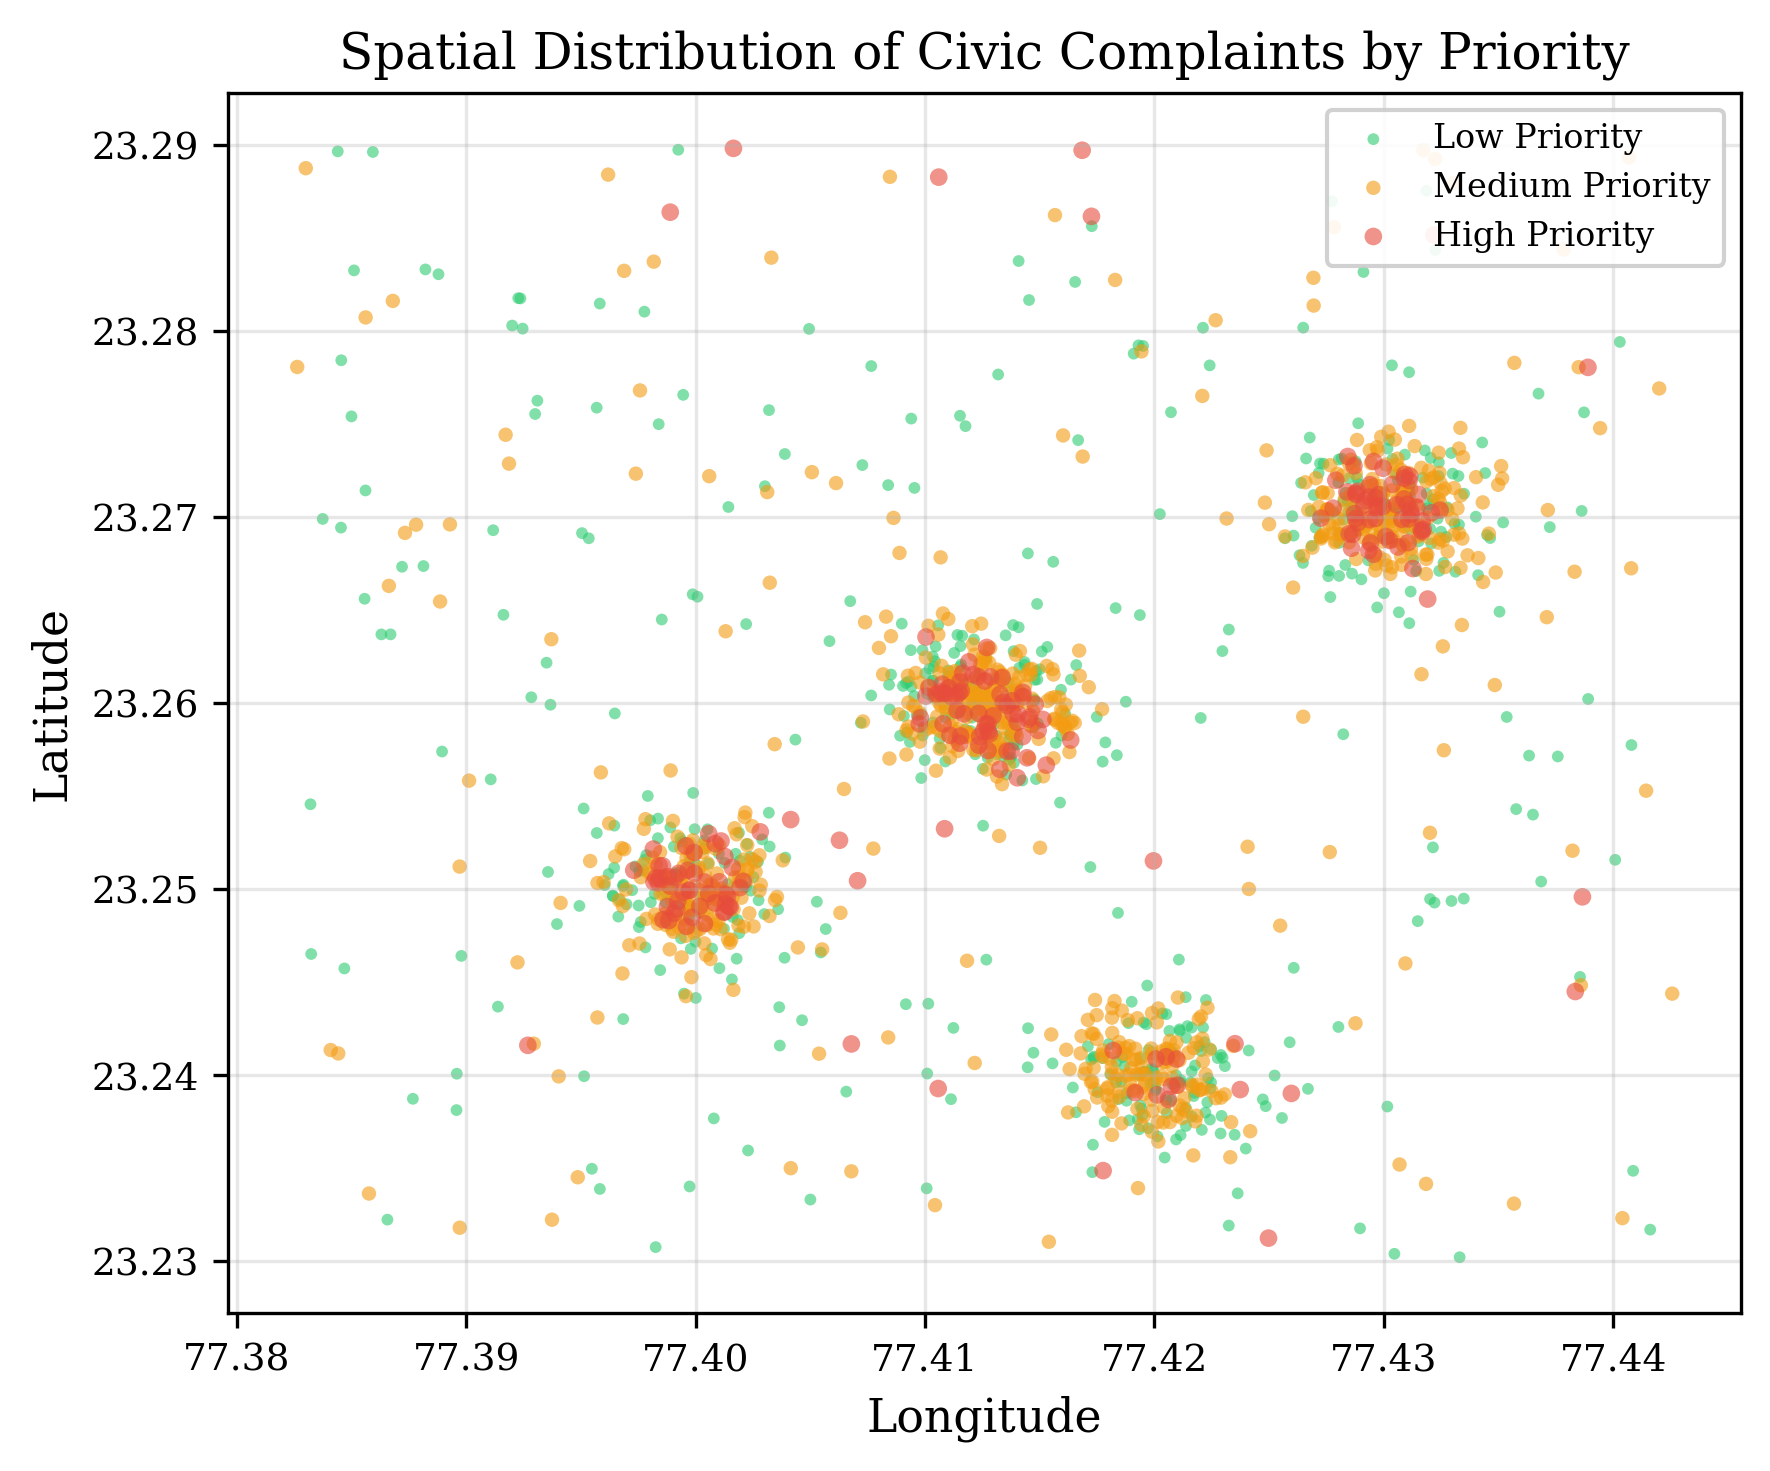
\includegraphics[width=0.45\textwidth]{../results/figures/spatial_distribution.png}
\caption{Spatial distribution of civic complaints by priority level.}
\label{fig:spatial_dist}
\end{figure}

\subsection{Priority Label Generation}

Priority labels are assigned using a composite scoring function that integrates domain knowledge with spatial context:

\begin{equation}
S = 0.4 \cdot S_{\text{cat}} + 0.3 \cdot W_{\text{status}} + 0.3 \cdot U_{\text{spatial}}
\end{equation}

where $S_{\text{cat}}$ is the normalized category severity (Water Supply: 1.0, Drainage: 0.8, Pothole: 0.6, Streetlight: 0.4, Waste: 0.2), $W_{\text{status}}$ is the status urgency weight (Pending: 1.0, Cancelled: 0.2, Completed: 0.0), and $U_{\text{spatial}}$ is the spatial urgency score.

The spatial urgency $U_{\text{spatial}}$ is computed as the normalized count of same-category complaints within a fixed labeling radius $r_l = 0.003^{\circ}$ ($\approx$330 meters):

\begin{equation}
U_{\text{spatial}}(i) = \frac{|\{j : j \neq i, \; d(i,j) < r_l, \; c_j = c_i\}|}{\max_k |\{j : j \neq k, \; d(k,j) < r_l, \; c_j = c_k\}|}
\end{equation}

where $d(i,j)$ is the Euclidean distance, $r_l = 0.003^{\circ}$, and $c_i$ denotes the complaint category. Labels are assigned as: High ($S \geq 0.7$), Medium ($0.4 \leq S < 0.7$), Low ($S < 0.4$). A 5\% random perturbation is applied to simulate labeling uncertainty.

\textbf{Avoiding circular dependencies:} The spatial urgency used for labeling counts same-category neighbors within a fixed radius---a fundamentally different metric from the KNN density feature used for classification (which measures distance to the $k_{\text{density}}=5$ nearest neighbors of \textit{any} category). This design ensures the model learns genuine spatial patterns rather than reverse-engineering its own labels.

\subsection{Feature Engineering}

Seven features are used for classification---five domain-engineered features plus two raw geographic coordinates:

\textbf{KNN Density Score:} Spatial density is computed using a $k$-nearest neighbors approach ($k_{\text{density}}=5$), where the average distance to the $k_{\text{density}}$ closest complaint locations is calculated:

\begin{equation}
\text{Density}(i) = \frac{1}{\frac{1}{k_{\text{density}}}\sum_{j \in \text{KNN}(i)} d(i,j) + \eta}
\end{equation}

where $\eta = 10^{-6}$ is a numerical regularization term that prevents division by zero. This distinguishes the regularization factor from the DBSCAN search radius parameter $\varepsilon_d$. Density values are min-max normalized to $[0, 1]$. This feature captures localized complaint concentration regardless of category.

\textbf{Category Encoding:} Label-encoded representation of the complaint category.

\textbf{Status Encoding:} Label-encoded representation of the resolution status.

\textbf{Category Frequency:} Frequency count of each complaint category across the training partition, capturing recurring issue types. During cross-validation, this statistic is recomputed on each training fold to avoid information leakage from the test partition.

\textbf{Pending Indicator:} Binary feature indicating whether a complaint is unresolved (status = ``Pending''). We note that this feature is a binary projection of the Status Encoding column; both are retained because the Random Forest benefits from the explicit binary signal, though future work could consolidate them.

\textbf{Geographic Coordinates:} Raw Latitude and Longitude values are included to provide fine-grained spatial positioning alongside the aggregated density score.

\subsection{Priority Classification}

Four classifiers are evaluated under identical class-weight balancing conditions:

\textbf{Logistic Regression (Baseline):} A class-balanced logistic regression model with 5,000 maximum iterations provides a linear baseline for comparison.

\textbf{Decision Tree:} A single decision tree with \texttt{max\_depth=6} and class-weight balancing is employed to model non-linear feature interactions.

\textbf{Random Forest:} An ensemble of 100 decision trees (\texttt{max\_depth=6}) with class-weight balancing is evaluated to reduce variance and improve generalization.

\textbf{XGBoost:} A gradient boosted decision tree classifier with maximum depth 6 is trained using sample weights to balance priority classes. The remaining XGBoost settings are left at library defaults.

All models are evaluated using stratified 5-fold cross-validation, an 80:20 stratified hold-out split, and a real-world validation set.

\subsection{Hotspot Detection}

Spatial clustering is performed using DBSCAN~\cite{ester1996dbscan} with a search radius parameter $\varepsilon_d = 0.002^{\circ}$ ($\approx$220 meters) and $\text{min\_samples} = 3$. DBSCAN is selected for its ability to identify arbitrarily-shaped clusters and handle noise---both common characteristics of urban spatial data.

Each detected cluster is assigned a composite risk level based on average density, pending complaint ratio, and high-priority complaint ratio, enabling identification of critical zones for targeted resource allocation.

\FloatBarrier
\section{Experiments and Results}

\subsection{Experimental Setup}

\textbf{Evaluation protocol:} Classification results are reported using stratified 5-fold cross-validation, summarized as mean $\pm$ standard deviation. Detailed per-class results use an 80:20 stratified hold-out split with random seed 42.

\textbf{Metrics:} Performance is measured using accuracy, macro-averaged F1-score, per-class precision/recall/F1, and ROC-AUC (one-vs-rest, macro-averaged).

\textbf{Hyperparameters:} Decision Tree and XGBoost use maximum depth 6. Random Forest uses 100 trees with maximum depth 6. Logistic Regression uses 5,000 maximum iterations. Class balancing is handled through class weights for scikit-learn models and sample weights for XGBoost. DBSCAN uses $\varepsilon_d=0.002$ and three minimum samples; KNN density uses $k_{\text{density}}=5$. All random seeds are fixed at 42.

\subsection{Model Comparison}

Table~\ref{tab:model_cv} presents the cross-validated performance comparison.

\begin{table}[t]
\centering
\caption{Model Performance --- 5-Fold Cross-Validation}
\label{tab:model_cv}
\resizebox{\columnwidth}{!}{%
\begin{tabular}{lcccc}
\toprule
Metric & Logistic Reg. & Decision Tree & Random Forest & XGBoost \\
\midrule
Accuracy & $0.678 \pm 0.046$ & $0.874 \pm 0.012$ & $0.903 \pm 0.017$ & $0.909 \pm 0.019$ \\
Macro F1 & $0.656 \pm 0.050$ & $0.844 \pm 0.016$ & $0.884 \pm 0.025$ & $0.885 \pm 0.030$ \\
ROC-AUC & 0.844 & 0.910 & 0.944 & 0.944 \\
p-val vs LR & -- & 0.0007 & 0.0004 & 0.0005 \\
\bottomrule
\end{tabular}}
\end{table}

The tree-based classifiers significantly outperform the linear logistic regression model across all metrics. Notably, the logistic regression model exhibits higher variance ($\pm 0.046$), suggesting greater sensitivity to non-linear interactions compared to the robust ensemble methods. Paired t-tests, performed on the five fold-wise cross-validation accuracies, verify that the accuracy improvements of the Decision Tree, Random Forest, and XGBoost models over the baseline are highly statistically significant ($p < 0.001$).

Table~\ref{tab:model_perclass} provides per-class hold-out results.

\begin{table}[h]
\centering
\caption{Per-Class Performance --- Hold-out Set}
\label{tab:model_perclass}
\setlength{\tabcolsep}{4.5pt}
\begin{tabular}{llccc}
\toprule
Model & Class & Precision & Recall & F1 \\
\midrule
\multirow{3}{*}{Logistic Reg.} & Low & 0.69 & 0.79 & 0.74 \\
 & Medium & 0.75 & 0.54 & 0.63 \\
 & High & 0.43 & 0.73 & 0.54 \\
\midrule
\multirow{3}{*}{Decision Tree} & Low & 0.85 & 0.91 & 0.88 \\
 & Medium & 0.92 & 0.80 & 0.86 \\
 & High & 0.62 & 0.83 & 0.71 \\
\midrule
\multirow{3}{*}{Random Forest} & Low & 0.83 & 0.93 & 0.88 \\
 & Medium & 0.93 & 0.83 & 0.88 \\
 & High & 0.79 & 0.85 & 0.82 \\
\midrule
\multirow{3}{*}{XGBoost} & Low & 0.87 & 0.94 & 0.90 \\
 & Medium & 0.93 & 0.87 & 0.90 \\
 & High & 0.80 & 0.83 & 0.81 \\
\bottomrule
\end{tabular}
\end{table}

The ensemble models achieve superior precision across all classes. Most notably, Random Forest and XGBoost dramatically improve the precision of the high-priority minority class (from 0.62 for DT to 0.79 for RF and 0.80 for XGBoost), mitigating the high rate of false positives that limits the single Decision Tree.

\begin{figure}[h]
\centering
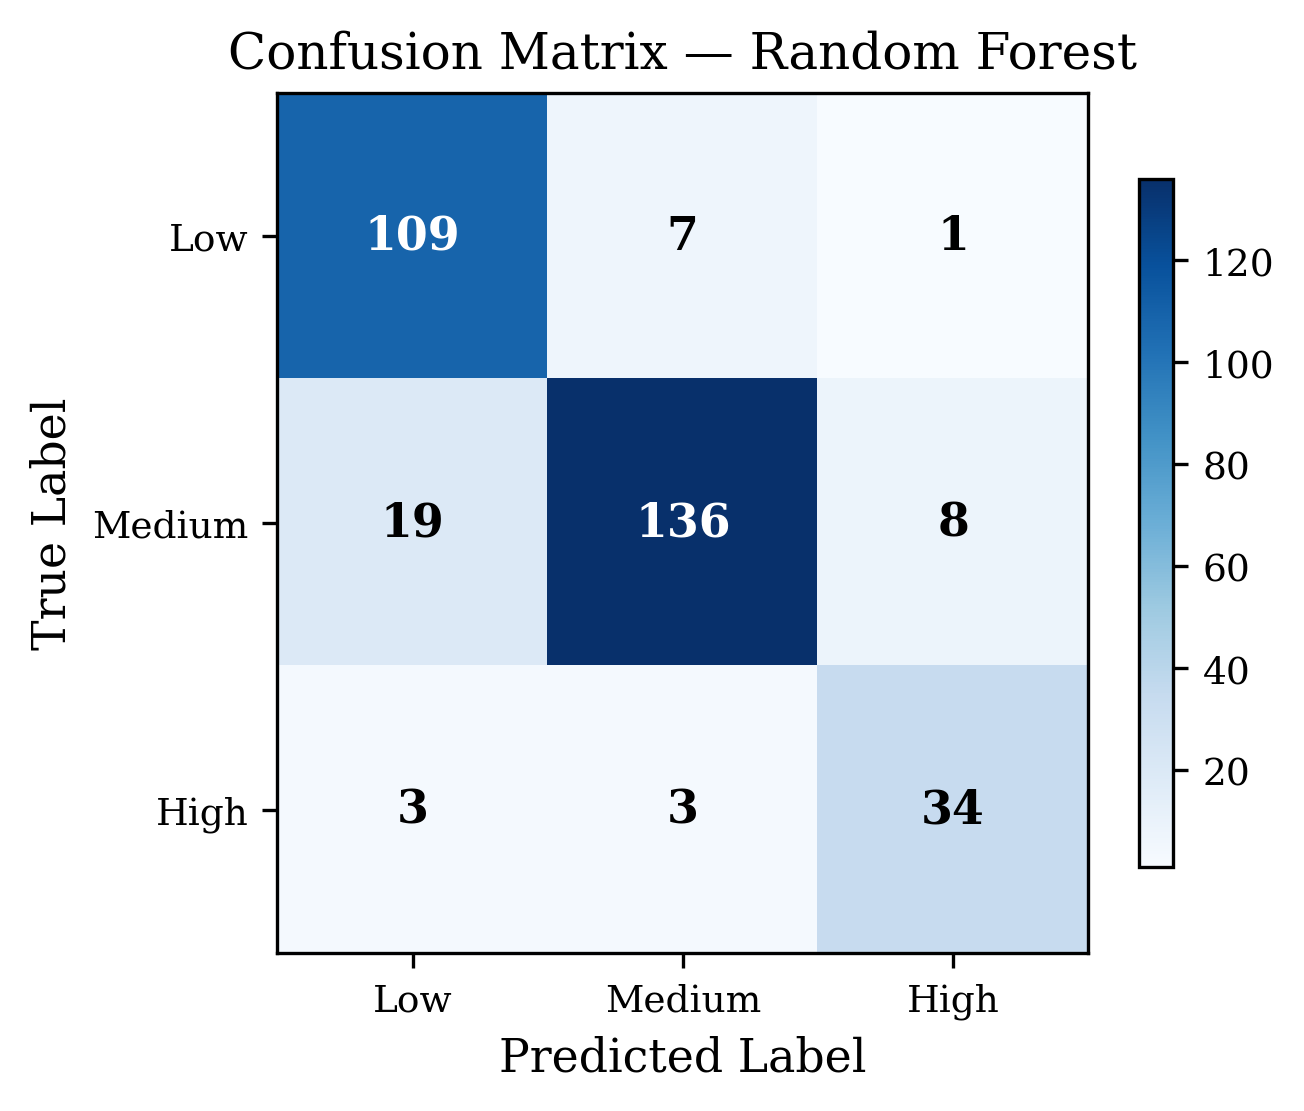
\includegraphics[width=0.45\textwidth]{../results/figures/confusion_matrix.png}
\caption{Confusion matrix of the Random Forest Classifier (hold-out set).}
\label{fig:confusion_matrix}
\end{figure}

The confusion matrix (Fig.~\ref{fig:confusion_matrix}) reveals that most misclassifications occur between adjacent priority levels (Low$\leftrightarrow$Medium, Medium$\leftrightarrow$High), consistent with the ordinal nature of the labels.

The ensemble models (Random Forest and XGBoost) achieve consistently higher one-vs-rest ROC-AUC values across all priority classes, with macro AUC reaching 0.944.

\subsection{Feature Importance Analysis}

Random Forest feature importance shows that the top three features are:
\begin{enumerate}
    \item \textbf{Status encoding} (0.194): Resolution status is the strongest predictor, reflecting the direct relationship between pending status and urgency.
    \item \textbf{Pending flag} (0.179): The binary flag indicating whether a ticket is unresolved is highly correlated with priority.
    \item \textbf{Category encoding} (0.174): The type of complaint (e.g., Water Supply vs. Waste) contributes significantly to the split decisions.
\end{enumerate}

The density score's consistent contribution (16.3\%), ranking fifth among the seven input features, validates the core hypothesis that spatial awareness meaningfully enhances prioritization alongside the top domain-knowledge predictors, even when labels are not directly derived from the density feature. Although status-related features rank highest individually, the ablation study demonstrates that removing spatial density causes a 12.9-percentage-point reduction in accuracy, confirming that density contributes complementary predictive information beyond status alone.

\subsection{Ablation Study}

To rigorously evaluate the contribution of spatial features, an ablation study is conducted by progressively adding features. All experiments use 5-fold stratified cross-validation on the Decision Tree classifier. The Decision Tree is chosen for the ablation because its single-tree structure isolates the impact of individual feature additions without ensemble averaging effects that could mask or smooth feature contributions.

\begin{table}[h]
\centering
\caption{Ablation Study --- Impact of Spatial Features}
\label{tab:ablation}
\resizebox{\columnwidth}{!}{%
\begin{tabular}{lccc}
\toprule
Feature Set & Accuracy & Macro F1 & High Recall \\
\midrule
Baseline (No Spatial) & $0.729 \pm 0.021$ & $0.710 \pm 0.019$ & 0.88 \\
+ Density & $0.858 \pm 0.025$ & $0.825 \pm 0.037$ & 0.83 \\
+ Density + Coords & $0.874 \pm 0.012$ & $0.844 \pm 0.016$ & 0.83 \\
\bottomrule
\end{tabular}}
\end{table}

\begin{figure}[h]
\centering
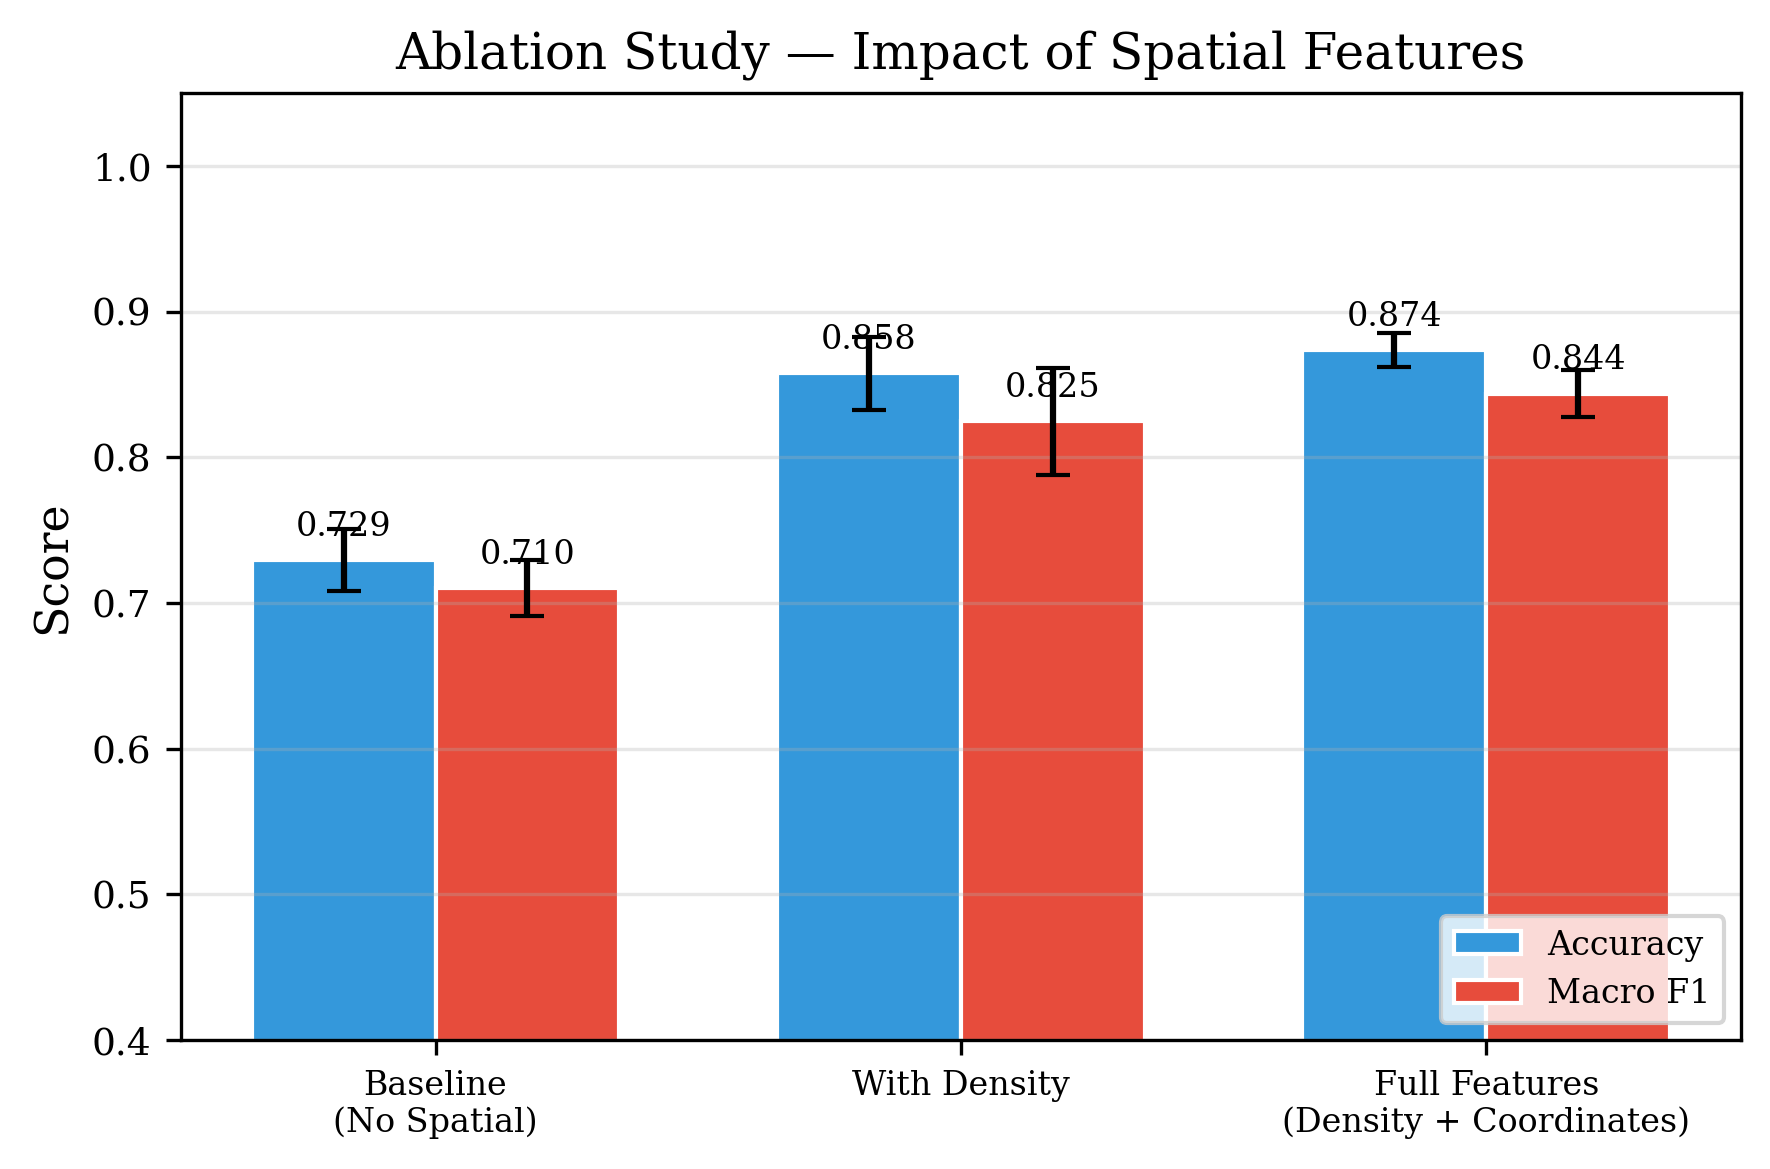
\includegraphics[width=0.45\textwidth]{../results/figures/ablation_accuracy.png}
\caption{Ablation study showing the impact of spatial features on accuracy and macro F1.}
\label{fig:ablation}
\end{figure}

The results demonstrate a substantial improvement from spatial features:

\begin{itemize}
    \item Adding density alone improves accuracy by \textbf{12.9 percentage points} (72.9\% $\to$ 85.8\%) and macro F1 by 11.5 points (0.710 $\to$ 0.825).
    \item Adding geographic coordinates provides a further 1.6-point accuracy gain (85.8\% $\to$ 87.4\%), with reduced variance ($\pm 0.012$ vs. $\pm 0.025$), indicating improved stability.
    \item The density feature alone accounts for \textbf{89\%} of the total spatial improvement, confirming that KNN density effectively captures the most relevant spatial information.
\end{itemize}

\textbf{Precision--Recall Trade-off for High-Urgency Class:} While incorporating spatial density features substantially boosts overall accuracy and macro F1, a slight decrease in the recall of the high-priority class is observed (from 0.88 to 0.83). Without spatial density features, the model lacks spatial context and overpredicts the High-priority class, resulting in high recall but a high rate of false positives (low precision of 0.49). When spatial density is included, the classifier learns a more nuanced decision boundary, which drastically reduces false positives---raising High-priority precision from 0.49 to 0.62 for Decision Tree, 0.79 for Random Forest, and 0.80 for XGBoost---at the minor cost of missing a few marginal cases. This represents a highly favorable trade-off for municipal dispatchers.

\subsection{Hotspot Analysis}

DBSCAN clustering identifies 28 spatial clusters from 1,600 complaint records, with 150 points classified as noise (9.4\%). The four largest clusters contain 86\% of all complaints, corresponding to major urban zones.

Table~\ref{tab:hotspots} summarizes the detected hotspot characteristics.

\begin{table}[h]
\centering
\caption{Top Hotspot Clusters by Complaint Volume}
\label{tab:hotspots}
\begin{tabular}{ccccl}
\toprule
Cluster & Count & Pending\% & Risk & Dominant Category \\
\midrule
0 & 409 & 47.9\% & LOW & Waste \\
2 & 362 & 50.8\% & LOW & Waste \\
3 & 314 & 49.7\% & LOW & Waste \\
4 & 264 & 49.2\% & LOW & Waste \\
20 & 3 & 100\% & MED & Pothole \\
25 & 3 & 66.7\% & MED & Drainage \\
\bottomrule
\end{tabular}
\end{table}

\begin{figure}[h]
\centering
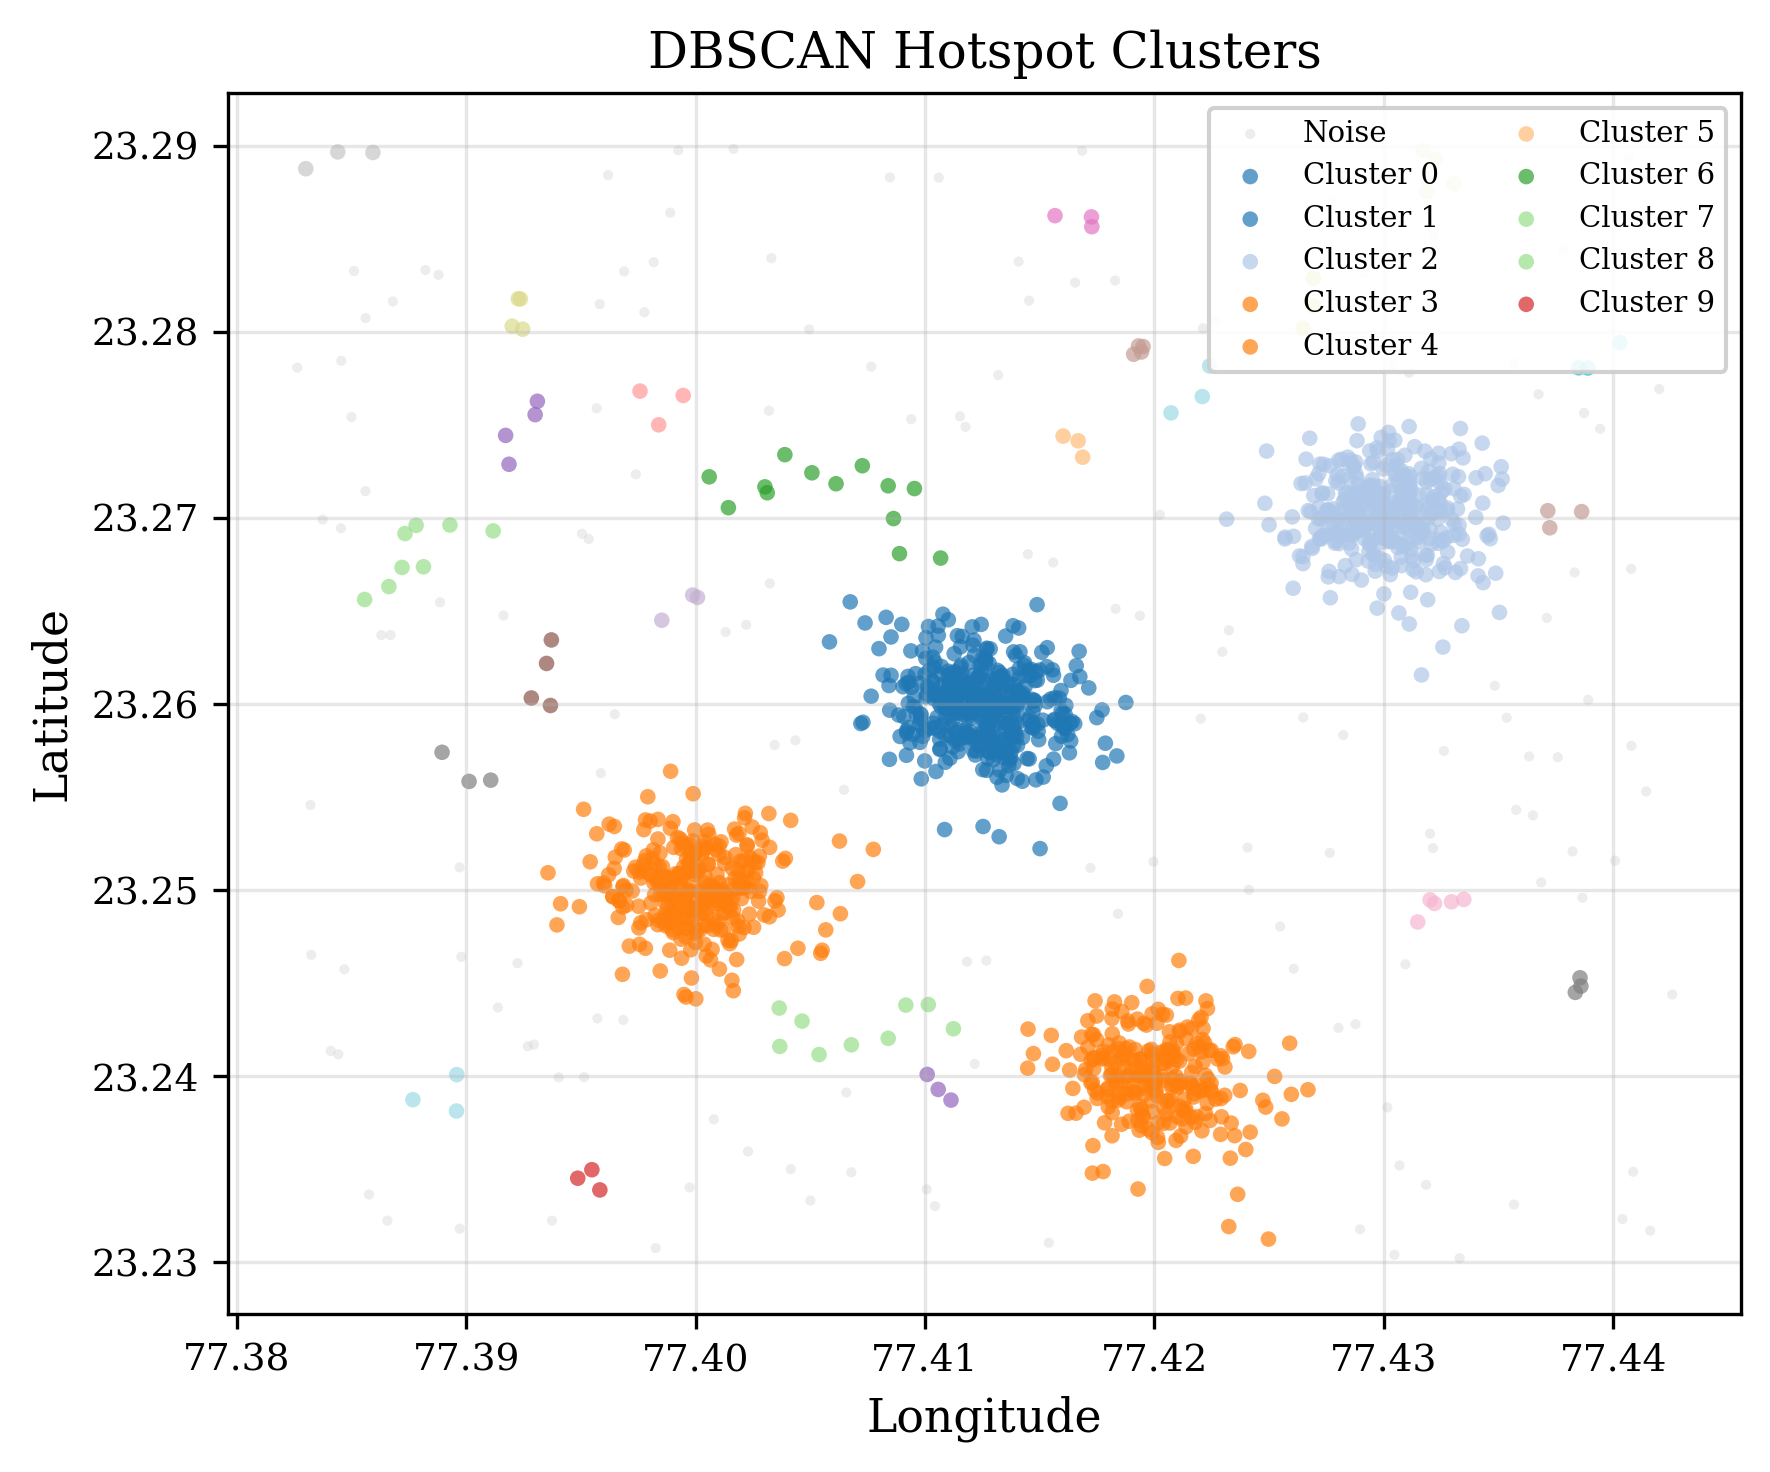
\includegraphics[width=0.45\textwidth]{../results/figures/hotspot_clusters.png}
\caption{DBSCAN hotspot clusters visualized spatially.}
\label{fig:hotspots}
\end{figure}

The clustering results (Fig.~\ref{fig:hotspots}) reveal that high-volume clusters are dominated by waste management complaints, while medium-risk clusters with smaller complaint counts contain a higher proportion of unresolved infrastructure issues (potholes, drainage). This spatial decomposition enables municipal authorities to allocate resources based on both complaint volume and urgency characteristics of each zone.

To strengthen the real-world spatial validation, the same DBSCAN-based hotspot analysis is also applied to the NYC~311 dataset. Using $\varepsilon_d=0.005^{\circ}$ and \texttt{min\_samples}=10, DBSCAN identifies 99 NYC clusters and 1,510 noise points from 5,469 records. Table~\ref{tab:nyc_hotspots} lists the highest-risk NYC hotspots and Fig.~\ref{fig:nyc_hotspots} visualizes the top 10 clusters.

\begin{table}[h]
\centering
\caption{Top NYC 311 Hotspots by DBSCAN Risk Score}
\label{tab:nyc_hotspots}
\begin{tabular}{ccccl}
\toprule
Cluster & Count & Pending\% & Risk & Dominant Category \\
\midrule
48 & 12 & 100.0\% & HIGH & Streetlight \\
75 & 10 & 60.0\% & HIGH & Streetlight \\
74 & 22 & 68.2\% & HIGH & Drainage \\
50 & 27 & 55.6\% & MED & Water Supply \\
58 & 18 & 77.8\% & MED & Water Supply \\
\bottomrule
\end{tabular}
\end{table}

\begin{figure}[h]
\centering
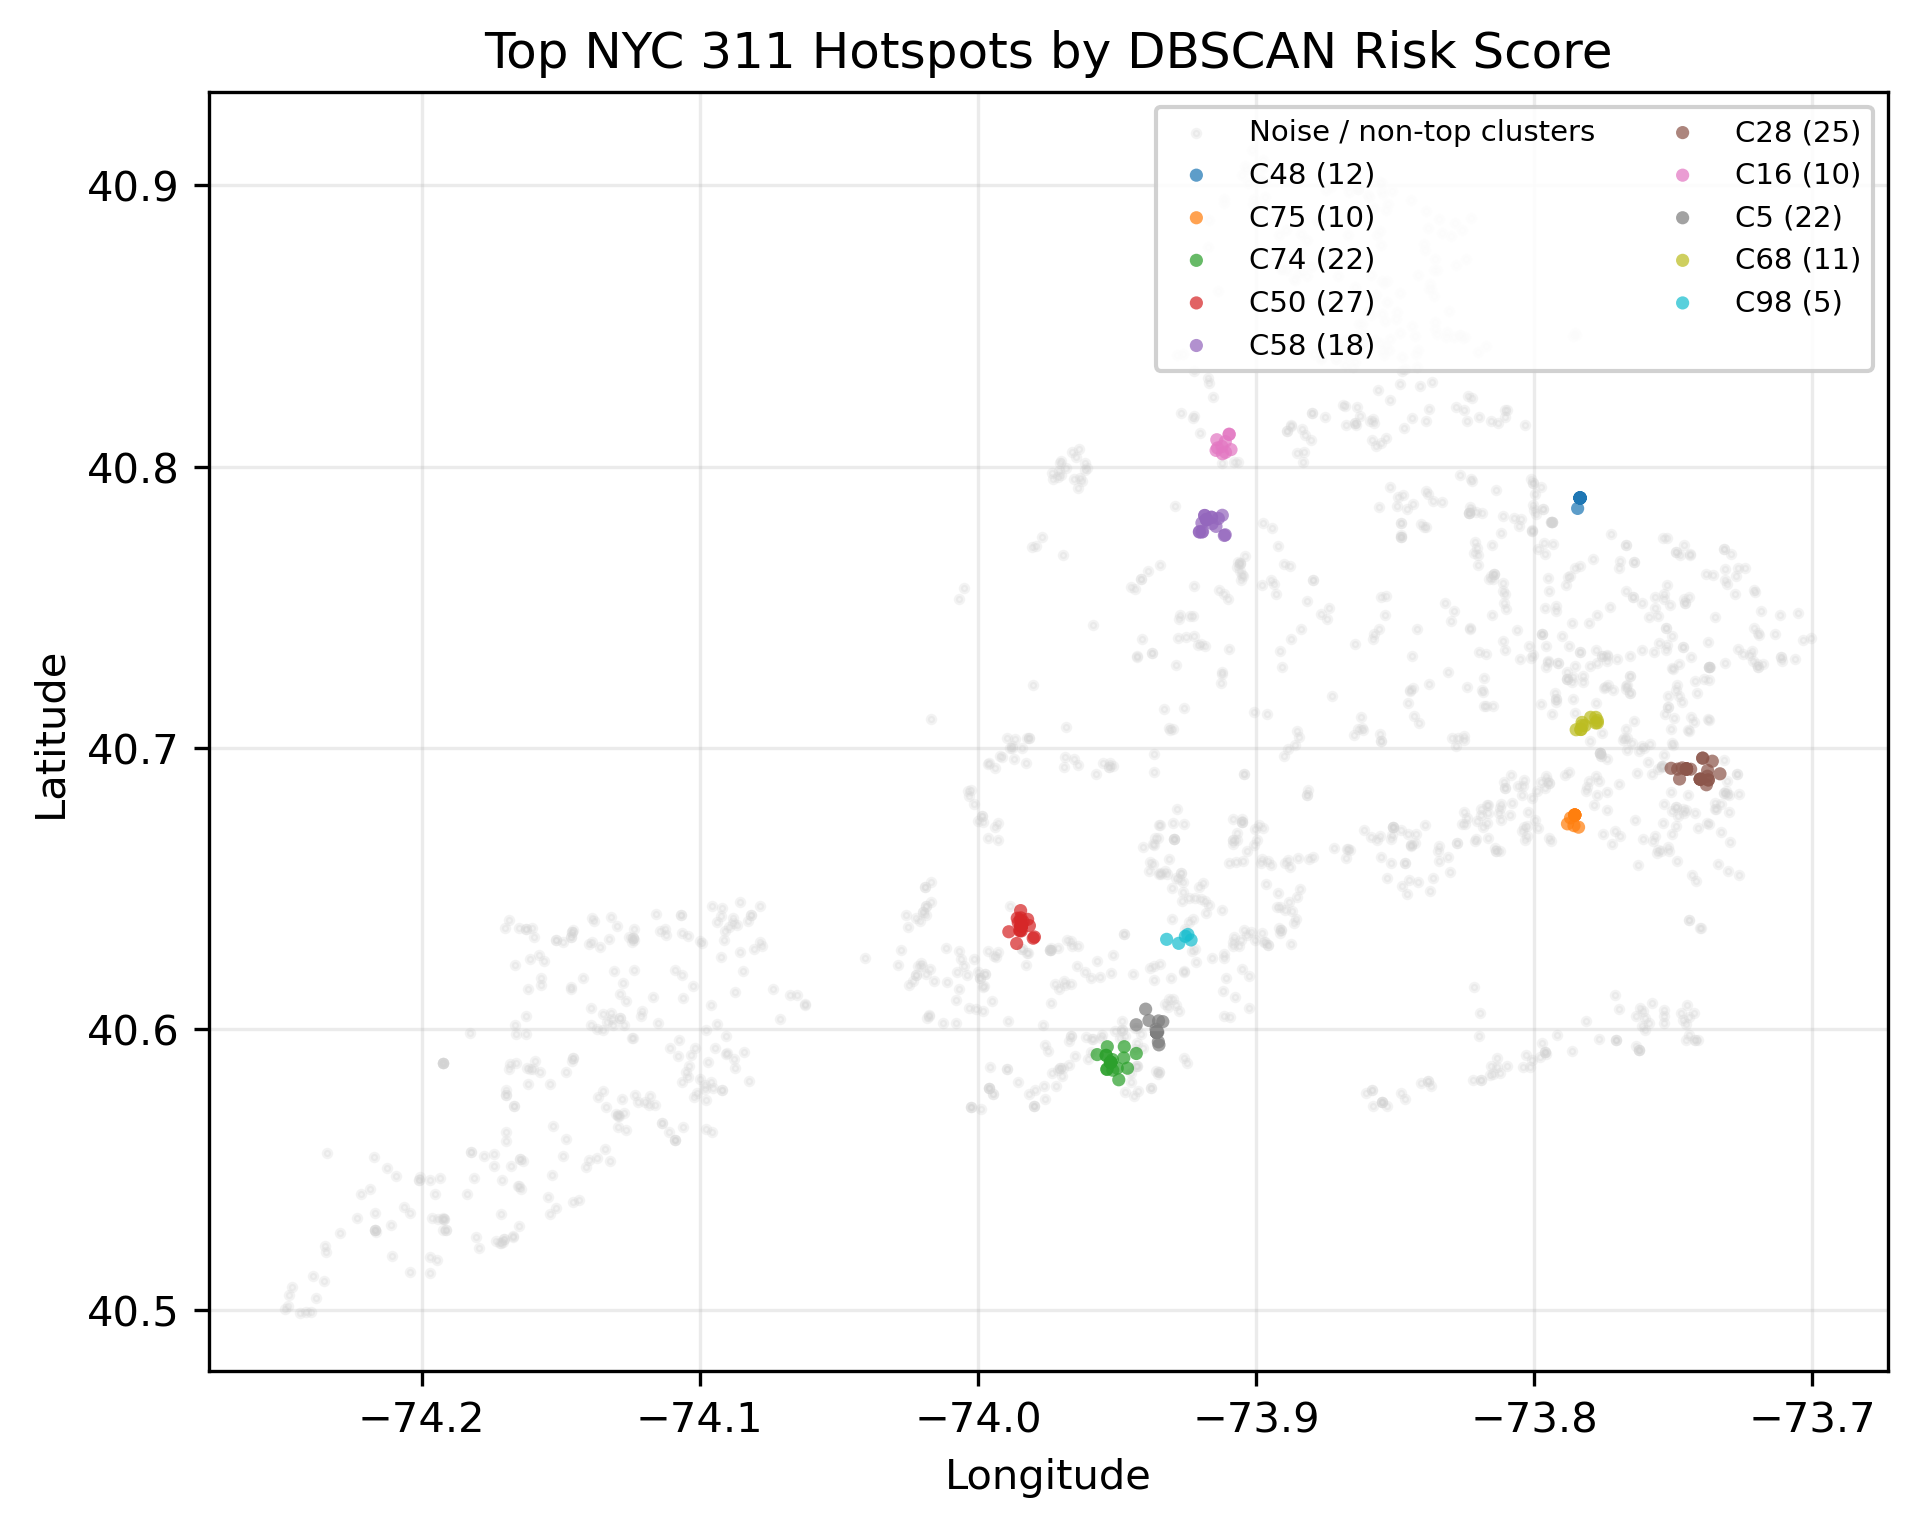
\includegraphics[width=0.48\textwidth]{../results/figures/nyc_hotspot_clusters.png}
\caption{Top NYC~311 hotspots detected using DBSCAN on real service-request coordinates.}
\label{fig:nyc_hotspots}
\end{figure}

The NYC hotspot map addresses the limitation that spatial clustering was previously demonstrated only on synthetic Bhopal data. The highest-risk NYC clusters are smaller but operationally meaningful, with several dominated by unresolved streetlight, drainage, and water-supply issues.

\subsection{Label Scoring Sensitivity Analysis}

To test whether Equation~(1) depends on a fragile weight choice, $w_1$, $w_2$, and $w_3$ are perturbed by $\pm 0.1$. Across all variants, the High-priority class remains non-empty (4.8\%--20.6\%) and Decision Tree cross-validated accuracy remains between 79.6\% and 91.5\%, indicating that the composite scoring function is not dominated by a single exact weight setting.

\subsection{Real-World Validation on NYC 311 Data}

To evaluate the framework beyond the controlled synthetic environment, two complementary experiments are conducted on real NYC~311 service request data.

\subsubsection{Zero-Shot Transfer (Bhopal $\to$ NYC)}

Classifiers trained on the Bhopal synthetic data are evaluated directly on a 600-record NYC~311 sample \textit{without retraining}. This deliberately tests the raw transferability of the spatial feature engineering. Table~\ref{tab:nyc311_zeroshot} presents the zero-shot results.

\begin{table}[h]
\centering
\caption{Zero-Shot Transfer --- Bhopal-Trained Models on NYC 311}
\label{tab:nyc311_zeroshot}
\begin{tabular}{lcc}
\toprule
Model & Accuracy & Macro F1 \\
\midrule
Logistic Regression & 38.8\% & 29.8\% \\
Decision Tree & 51.5\% & 43.6\% \\
Random Forest & 65.3\% & 45.9\% \\
XGBoost & 38.7\% & 28.4\% \\
\bottomrule
\end{tabular}
\end{table}

Random Forest exceeds random chance (33.3\%) by 32 percentage points, confirming that spatial feature representations transfer meaningfully for non-linear models, but the performance decline from the source domain highlights a severe domain shift driven by differences in city layout, reporting volume, and label semantics. XGBoost's sensitivity to source-domain feature distributions makes it more susceptible to domain shift than the bagged Random Forest ensemble, which generalizes more robustly across geographic contexts.

\subsubsection{Direct NYC Training with Outcome-Based Labels}

To directly address the synthetic-data criticism, all four classifiers are retrained and evaluated on 5,469 real NYC~311 records using outcome-based priority labels derived from observed resolution latency (Section~III-B). The same seven-feature pipeline is applied identically to the NYC data. Table~\ref{tab:nyc311_direct} reports 5-fold cross-validated performance.

\begin{table}[h]
\centering
\caption{Direct NYC 311 Training --- 5-Fold Cross-Validation}
\label{tab:nyc311_direct}
\begin{tabular}{lccc}
\toprule
Model & Accuracy & Macro F1 & p-val vs LR \\
\midrule
Logistic Reg. & $0.942 \pm 0.004$ & $0.880 \pm 0.008$ & -- \\
Decision Tree & $0.950 \pm 0.003$ & $0.894 \pm 0.006$ & 0.014 \\
Random Forest & $0.952 \pm 0.002$ & $0.897 \pm 0.005$ & 0.005 \\
XGBoost & $0.957 \pm 0.002$ & $0.903 \pm 0.005$ & 0.006 \\
\bottomrule
\end{tabular}
\end{table}

All tree-based models significantly outperform the LR baseline (paired t-tests on five fold-wise accuracies, $p < 0.05$). XGBoost achieves 95.7\% accuracy and 0.903 macro F1 on real outcome-labeled data, confirming that the spatial feature pipeline can be trained successfully beyond synthetic labels. This high NYC performance is interpreted cautiously because outcome-based labels are partially correlated with complaint status, potentially simplifying the classification task.

\textbf{NYC hold-out per-class performance:} On a stratified 80:20 hold-out split (1,094 test records), XGBoost achieves per-class F1 scores of 0.997 (Low), 0.907 (Medium), and 0.789 (High), with ROC-AUC = 0.992. The High-priority recall of 0.86 indicates that outcome-based labels produce a more balanced classification problem than Equation~1 labels, where High-priority precision was the primary bottleneck.

\textbf{Real-world ablation:} To test whether spatial information remains useful on NYC data, a compact ablation is performed using the Decision Tree classifier. The non-spatial baseline achieves $0.942 \pm 0.004$ accuracy and $0.880 \pm 0.008$ macro F1. Adding KNN density alone yields $0.940 \pm 0.003$ accuracy and $0.877 \pm 0.007$ macro F1, while adding both density and raw coordinates improves performance to $0.950 \pm 0.003$ accuracy and $0.894 \pm 0.006$ macro F1. Thus, unlike the controlled Bhopal experiment where density alone drives most of the gain, NYC benefits from the combination of local density and absolute geographic position. The marginal decrease when adding density alone suggests that on NYC data, absolute geographic position is the primary spatial carrier, with KNN density providing complementary local contrast only when combined with coordinates.

\textbf{Status and density robustness:} Because outcome-based NYC labels are correlated with complaint status, an additional XGBoost feature-removal test is conducted. Using all features yields $0.957 \pm 0.002$ accuracy and $0.903 \pm 0.005$ macro F1. Removing status-related features reduces performance to $0.799 \pm 0.007$ accuracy and $0.754 \pm 0.010$ macro F1, confirming that administrative status is a strong predictor. Removing only density has a smaller effect ($0.955 \pm 0.003$ accuracy and $0.899 \pm 0.006$ macro F1), showing that density is complementary rather than dominant on NYC. Random Forest feature importance on NYC tells the same story: status encoding (0.278), pending flag (0.257), category frequency (0.223), category encoding (0.175), latitude (0.028), longitude (0.027), and density (0.013).

\subsubsection{Cross-Dataset Comparison}

Table~\ref{tab:cross_dataset} consolidates results across datasets and label sources, demonstrating that the framework performs consistently across both controlled and real-world conditions.

\begin{table}[h]
\centering
\caption{Cross-Dataset Comparison}
\label{tab:cross_dataset}
\setlength{\tabcolsep}{3pt}
\begin{tabular}{llccc}
\toprule
Dataset & Label Source & Model & Accuracy & Macro F1 \\
\midrule
Synthetic Bhopal & Eq.~1 scoring & XGB & 90.9\% & 88.5\% \\
NYC 311 (direct) & Outcome proxy & XGB & 95.7\% & 90.3\% \\
NYC 311 (zero-shot) & Eq.~1 transfer & RF & 65.3\% & 45.9\% \\
\bottomrule
\end{tabular}
\end{table}

The contrast between direct NYC training (95.7\%) and best zero-shot transfer (65.3\%) confirms that the feature engineering pipeline is useful but region-specific. Practical deployment therefore requires local calibration rather than direct model reuse across cities.

\section{Discussion}

\subsection{Key Findings}

Four observations emerge consistently across the experiments:

\textbf{(1) Spatial density is useful, but its contribution is dataset-dependent.} The synthetic Bhopal ablation shows that KNN density is a strong independent signal, improving Decision Tree accuracy by 12.9 percentage points (72.9\% $\to$ 87.4\%). On NYC, density alone slightly reduces performance, while density plus coordinates improves accuracy from 94.2\% to 95.0\%. This contrast is an important finding: controlled synthetic data isolates local concentration effects, whereas real NYC data depends more heavily on absolute geographic position, with density acting as a complementary local-contrast feature. The substantially lower density importance observed on NYC data (0.013 versus 0.163 in the synthetic environment) likely reflects differences in spatial organization: the synthetic Bhopal dataset was designed around localized reporting clusters, while NYC complaints are distributed across a larger and more heterogeneous urban landscape.

\textbf{(2) Ensemble tree-based models outperform linear models for spatial civic data.} XGBoost achieves 90.9\% accuracy on the synthetic Bhopal dataset and 95.7\% on the NYC 311 dataset, compared to 67.8\% and 94.2\% respectively for logistic regression under identical conditions. This performance gap reflects the inherently non-linear interactions between spatial, categorical, and status features. The ensemble models also dramatically improve the precision of the minority high-priority class.

\textbf{(3) The feature pipeline generalizes to real-world data with outcome-based labels.} Training directly on 5,469 NYC 311 records labeled by observed resolution latency, XGBoost achieves 95.7\% accuracy and 0.903 macro F1 (Table~\ref{tab:nyc311_direct}). This confirms that the feature engineering pipeline can be trained effectively on real municipal complaint data. The higher absolute accuracy on NYC compared to the synthetic dataset (95.7\% vs.\ 90.9\%) likely reflects the larger dataset size and stronger label--status correlation in outcome-based labels.

\textbf{(4) Direct model transfer remains difficult.} Zero-shot transfer from Bhopal to NYC reaches 65.3\% accuracy with Random Forest, while XGBoost drops to 38.7\%. Direct NYC training with the same seven-feature pipeline reaches 95.7\%. This gap confirms that spatial features are useful but require regional calibration because label definitions, geographic distributions, and reporting behavior differ substantially across cities.

\subsection{Limitations}

A practical limitation of the present study is that several design choices remain tied to the available data:

\textbf{Synthetic dataset as primary controlled environment:} The Bhopal dataset is synthetically generated, meaning labels, spatial patterns, and class distributions are artificial. While NYC 311 direct training and hotspot analysis confirm that the pipeline can operate on real data, the sensitivity analysis is conducted only on the synthetic dataset. Reproducing sensitivity tests on large-scale real municipal data remains future work.

\textbf{Outcome-based label proxy:} The NYC 311 priority labels use resolution latency as a proxy for urgency. This conflates slow bureaucratic processing with genuine high-severity issues and is partially correlated with complaint status, which may simplify the direct NYC classification task. Human-annotated ground truth (e.g., expert labels with inter-annotator agreement via Cohen's Kappa) would provide a more rigorous validation target.

\textbf{Cross-city generalization:} While the framework is validated on both Bhopal (synthetic) and NYC (real) data, cross-city transfer---training on one city and testing on another---remains an open challenge, as demonstrated by the zero-shot transfer results. Multi-city generalization studies (e.g., incorporating Chicago 311 data) are left to future work.

\textbf{Hyperparameter sensitivity:} Key parameters---DBSCAN search radius $\varepsilon_d$, same-category labeling radius $r_l$, and KNN density $k_{\text{density}}$---are fixed without systematic optimization. Future work should explore hyperparameter sensitivity and automated tuning.

\textbf{Temporal dynamics:} The current framework treats complaints as a static snapshot. Real-world prioritization should incorporate temporal features such as complaint age, resolution velocity, and seasonal patterns.

\textbf{Feature redundancy:} The Status Encoding and Pending Indicator features encode overlapping information from the same resolution-status column. While both are retained because the explicit binary signal marginally improves tree split efficiency, their joint high importance (0.194 and 0.179) may inflate the apparent contribution of status-related attributes relative to other features.

\section{Conclusion}

This paper presents a spatially-aware machine learning framework for prioritizing urban civic complaints using density-based feature engineering. By integrating KNN-based spatial density, domain-knowledge labeling, and DBSCAN hotspot detection, the framework captures both individual-level urgency and zone-level spatial patterns. A hybrid dataset strategy---combining a synthetic Bhopal dataset for controlled experimentation with real NYC~311 data for external validation---addresses the inherent limitations of purely synthetic evaluation.

On the synthetic dataset, the ablation study demonstrates that density-based features improve Decision Tree classification accuracy by 12.9 percentage points, establishing spatial awareness as a critical component of civic prioritization systems. On real NYC~311 data with outcome-based labels, XGBoost achieves 95.7\% cross-validated accuracy with 0.992 ROC-AUC, although this result should be interpreted with care due to the status--outcome relationship in the labels. DBSCAN clustering identifies 28 controlled Bhopal hotspots and 99 NYC hotspots, enabling targeted municipal resource allocation.

Future work will focus on: (1) cross-city generalization studies using additional municipal datasets (e.g., Chicago 311) to evaluate urban transferability; (2) human-annotated ground-truth labels with inter-annotator agreement metrics to replace proxy labels; (3) incorporation of temporal features (complaint age, seasonality, repeat complaints) for dynamic priority adjustment; and (4) deployment as a real-time decision support module within smart city platforms~\cite{gharaibeh2017smart}.

The findings reinforce the importance of integrating spatial intelligence into automated urban management systems, demonstrating that density-based features yield substantial improvements in civic complaint prioritization on both synthetic and real-world municipal data.

\section*{Data Availability}
The code and synthetic Bhopal dataset used in this study will be made available upon acceptance at a public GitHub repository. The NYC 311 data is sourced from the NYC Open Data Socrata API (\url{https://data.cityofnewyork.us/}). The outcome-based label generation script and direct NYC training pipeline are included in the repository.

\bibliographystyle{IEEEtran}
\bibliography{references}

\end{document}
